\documentclass[12pt]{article}


\usepackage[english]{babel}
\usepackage[utf8]{inputenc}
\usepackage{amsmath,amssymb}
\usepackage{listings} % untuk kode python
\usepackage{xcolor}

\definecolor{codegreen}{rgb}{0,0.6,0}
\definecolor{codegray}{rgb}{0.5,0.5,0.5}
\definecolor{codepurple}{rgb}{0.58,0,0.82}
\definecolor{backcolour}{rgb}{0.95,0.95,0.92}

\lstdefinestyle{mystyle}{
    backgroundcolor=\color{backcolour},   
    commentstyle=\color{codegreen},
    keywordstyle=\color{magenta},
    numberstyle=\tiny\color{codegray},
    stringstyle=\color{codepurple},
    basicstyle=\ttfamily\footnotesize,
    breakatwhitespace=false,         
    breaklines=true,                 
    captionpos=b,                    
    keepspaces=true,                 
    numbers=left,                    
    numbersep=5pt,                  
    showspaces=false,                
    showstringspaces=false,
    showtabs=false,                  
    tabsize=2
}

\lstset{style=mystyle}
%\usepackage{parskip}
\usepackage{graphicx}

% Margins
\usepackage[top=2.5cm, left=3cm, right=3cm, bottom=4.0cm]{geometry}
\usepackage{hyperref}
\usepackage{natbib}
\usepackage{comment}
\setlength\bibsep{1em}
\setlength\bibhang{1.5em}
\renewcommand\bibfont{\singlespace}
\bibliographystyle{dcu}
% Colour table cells
%\usepackage[table]{xcolor}

% Get larger line spacing in table
\newcommand{\tablespace}{\\[1.25mm]}
\newcommand\Tstrut{\rule{0pt}{2.6ex}}         % = `top' strut
\newcommand\tstrut{\rule{0pt}{2.0ex}}         % = `top' strut
\newcommand\Bstrut{\rule[-0.9ex]{0pt}{0pt}}   % = `bottom' strut

%%%%%%%%%%%%%%%%%
%     Title     %
%%%%%%%%%%%%%%%%%
\title{Exercise 3 - Multi-class Classification and Neural Networks}
\author{Azka NA}
\date{\today}

\begin{document}
\maketitle

%%%%%%%%%%%%%%%%%
%   Problem 1   %
%%%%%%%%%%%%%%%%%

\section{Introduction}
This is the guide for Andrew Ng's Machine Learning course programming assignment done in Python, adapted from the original guide written for Octave or MATLAB.

In this exercise, you will implement  one-vs-all logistic regression and neural networks to recognize hand-written digits. Before starting on this programming exercise, we strongly recommend watching the video lectures and completing the review questions for the associated topics

For Programming Exercise 3: Multi-class Classification and Neural Networks, you will need to download the following files:

\texttt{exercise3.ipynb} - Jupyter notebook containing the script

\texttt{ex3data1.mat} - Training set of hand-written digits

\texttt{ex3weights.mat} - Initial weights for the neural network exercise

\hrulefill

\section{Multi-class Classification}

For this exercise, you will use logistic regression and neural networks to recognize handwritten digits (from 0 to 9). Automated handwritten digit recognition is widely used today - from recognizing zip codes (postal codes) on mail envelopes to recognizing amounts written on bank checks. This exercise will show you how the methods you’ve learned can be used for this classification task.

In the first part of the exercise, you will extend your previous implementation of logistic regression and apply it to one-vs-all classification.

\subsection{Dataset}

You are given a data set in \texttt{ex3data1.mat} that contains 5000 training examples of handwritten digits.\footnote{This is a subset of the MNIST handwritten digit dataset (\href{http://yann.lecun.com/exdb/mnist/}{http://yann.lecun.com/exdb/mnist/}).} The \texttt{.mat} format means that that the data has been saved in a native Octave/MATLAB matrix format, instead of a text (ASCII) format like a csv-file. These matrices can be read directly into your program by using the \texttt{load} function from \texttt{scipy.io}. After loading, matrices of the correct dimensions and values will appear in your program’s memory. The matrix will already be named, so you do not need to assign names to them.

\begin{lstlisting}[language=Python]
  from scipy.io import loadmat
  data = loadmat('ex3data1.mat')
  X_raw = data['X']
  y = data['y']
\end{lstlisting}

There are 5000 training examples in \texxttt{ex3data1.mat}, where each training example is a 20 pixel by 20 pixel grayscale image of the digit. Each pixel is represented by a floating point number indicating the grayscale intensity at that location. The 20 by 20 grid of pixels is "unrolled" into a 400-dimensional vector. Each of these training examples becomes a single row in our data matrix X. This gives us a 5000 by 400 matrix X where every row is a training example for a handwritten digit image, each with 400 features from its 20 x 20 pixel.

\begin{align}
  \mathbf {}X = \begin{bmatrix} \text{--- }(x^{(1)})^T \text{ ---} \\ \text{--- }(x^{(2)})^T \text{ ---} \\ \vdots \\ \text{--- }(x^{(m)})^T \text{ ---} \end{bmatrix}
\end{align}

The second part of the training set is a 5000-dimensional vector y that contains labels for the training set. In the given dataset, each training example has a label ranging from 1 to 10, a "0" digit is labeled as "10", while the digits "1" to "9" are labeled as "1" to "9" in their natural order.

\subsection{Visualizing the data}

You will begin by visualizing a subset of the training set. In the code below\footnote{The code for the plot from \href{https://medium.com/analytics-vidhya/a-guide-to-using-logistic-regression-for-digit-recognition-with-python-codes-86aae6da10fe}{here}}, we randomly select 100 rows out of total 5000 training examples. Then we map each row to a 20 pixel by 20 pixel image and displays the images together. 

\begin{lstlisting}
  _, axarr = plt.subplots(10,10,figsize=(10,10))
  for i in range(10):
      for j in range(10):
         axarr[i,j].imshow(X_raw[np.random.randint(X_raw.shape[0])].\
  reshape((20,20), order = 'F'))          
         axarr[i,j].axis('off') 
\end{lstlisting}

The result is Figure~\ref{fig:digits}.

\begin{figure}[h!]
  \centering
  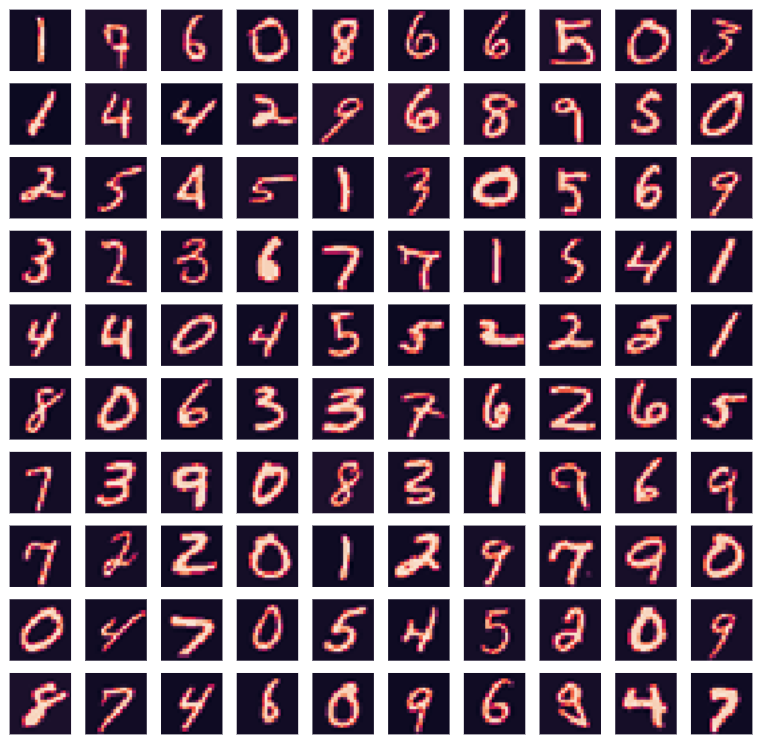
\includegraphics[scale=0.4]{digits.png}
  \caption{Examples from the dataset}
  \label{fig:digits}
\end{figure}

\subsection{Vectorizing Logistic Regression}

You will be using multiple one-vs-all logistic regression models to build a multi-class classifier. Since there are 10 classes, you will need to train 10 separate logistic regression classifiers. To make this training efficient, it is important to ensure that your code is well vectorized. In this section, you will implement a vectorized version of logistic regression that does not employ any for loops. You can use your code in the last exercise as a starting point \texttt{for} this exercise.

\subsubsection{Vectorizing the cost function}

We will begin by writing a vectorized version of the cost function. Recall that in (unregularized) logistic regression, the cost function is

\begin{align}
  J(\theta) & = \frac{1}{m}\sum_{i=1}^m{\big[-y^{(i)}log(h_\theta(x^{(i)}))-(1-y^{(i)}log(1-h_\theta(x^{(i)})))\big]}
\end{align}

To compute each element in the summation, we have to compute $h_\theta(x^{(i)})$ for every example $i$, where $h_\theta(x^{(i)}) = g(\theta^Tx^{(i)})$ and $g(z) = \frac{1}{1+e^{-z}}$ is the sigmoid function. It turns out that we can compute this quickly for all our examples by using matrix multiplication. Let us define $X$ and $\theta$ as


\begin{align}
  \mathbf {}X = \begin{bmatrix} \text{--- }(x^{(1)})^T \text{ ---} \\ \text{--- }(x^{(2)})^T \text{ ---} \\ \vdots \\ \text{--- }(x^{(m)})^T \text{ ---} \end{bmatrix} \text{ and } \theta = \begin{bmatrix} \theta_0 \\ \theta_1 \\ \vdots \\ \theta_n \end{bmatrix} .
\end{align}

Then, by computing the matrix product $X\theta$, we have

\begin{align}
  \mathbf {}X = \begin{bmatrix} \text{--- }(x^{(1)})^T\theta \text{ ---} \\ \text{--- }(x^{(2)})^T\theta \text{ ---} \\ \vdots \\ \text{--- }(x^{(m)})^T\theta \text{ ---} \end{bmatrix} = \begin{bmatrix} \text{--- }\theta^T(x^{(1)}) \text{ ---} \\ \text{--- }\theta^T(x^{(2)}) \text{ ---} \\ \vdots \\ \text{--- }\theta^T(x^{(m)}) \text{ ---} \end{bmatrix} .
\end{align}

In the last equality, we used the fact that $a^Tb = b^Ta$ if $a$ and $b$ are vectors. This allows us to compute the products $\theta^Tx^{(i)}$ for all our examples $i$ in one line of code.

Below is the code for \texttt{costFunctionReg}:

\begin{lstlisting}[language=Python]
  def costFunctionReg(theta, X, y, lmbd):
    m = len(y)
    z = np.dot(X, theta)
    term1 = np.multiply(-y, np.log(sigmoid(z)))
    term2 = np.multiply((1-y), np.log(1-sigmoid(z)))
    J = (1/m)*np.sum(term1 - term2) + lmbd/(2*m)*np.sum(theta[1:]**2)
    return J
\end{lstlisting}

\subsubsection{Vectorizing the gradient}

Recall that the gradient of the (unregularized) logistic regression cost is a vector where the $j^{th}$ element is defined as

\begin{align}
  \frac{\partial J}{\partial \theta_j} = \frac{1}{m}\sum_{i=1}^m{\big((h_\theta(x^{(i)})-y^{(i)})x_j^{(i)}\big)}
\end{align}

To vectorize this operation over the dataset, we start by writing out all the partial derivatives explicitly for all $\theta_j$,

\begin{align}
  \label{eq:vector}
   \begin{bmatrix} \frac{\partial J}{\partial \theta_0} \\[0.5em] \frac{\partial J}{\partial \theta_1} \\[0.5em] \frac{\partial J}{\partial \theta_2} \\[0.5em] \vdots \\[0.5em] \frac{\partial J}{\partial \theta_n} \end{bmatrix} & = \frac{1}{m} \begin{bmatrix} \sum_{i=1}^m{\big((h_\theta(x^{(i)})-y^{(i)})x_0^{(i)}\big)} \\[0.5em]\sum_{i=1}^m{\big((h_\theta(x^{(i)})-y^{(i)})x_1^{(i)}\big)} \\[0.5em] \sum_{i=1}^m{\big((h_\theta(x^{(i)})-y^{(i)})x_2^{(i)}\big)} \\[0.5em] \vdots \\[0.5em] \sum_{i=1}^m{\big((h_\theta(x^{(i)})-y^{(i)})x_0^{(n)}\big)} \end{bmatrix} \\[0.5em]
  & = \frac{1}{m}\sum_{i=1}^m{((h_\theta(x^{(i)})-y^{(i)})x^{(i)})} \\
  & = \frac{1}{m}X^T(h_\theta(x) - y).
\end{align}

where

\begin{align}
  h_\theta(x) - y = \begin{bmatrix} h_\theta(x^{(1)}) - y^{(1)} \\ h_\theta(x^{(2)}) - y^{(2)} \\ \vdots \\ h_\theta(x^{(m)}) - y^{(m)}  \end{bmatrix}
\end{align}

Note that $x^{(i)}$ is a vector, while $(h_\theta(x^{(i)}) - y^{(i)})$ is a scalar (single number). To understand the last step of the derivation, let $\beta_i = (h_\theta(x^{(i)}) - y^{(i)})$ and observe that:

\begin{align}
  \sum_{i}{\beta_i x^{(i)}} = \begin{bmatrix} \text{\textbar} & \text{\textbar} & & \text{\textbar} \\
  x^{(1)} & x^{(2)} & \cdots & x^{(m)} \\
  \text{\textbar} & \text{\textbar} & & \text{\textbar} 
  \end{bmatrix}
  \begin{bmatrix}
    \beta_1 \\ \beta_2 \\ \vdots \\ \beta_m
  \end{bmatrix} = X^T \beta\text{,}
\end{align}

where the values $\beta_i = (h_\theta(x^{(i)}) - y^{(i)})$.

The expression above allows us to compute all the partial derivatives without any loops. If you are comfortable with linear algebra, we encourage you to work through the matrix multiplications above to convince yourself that the vectorized version does the same computations. You should now implement Equation~\ref{eq:vector} to compute the correct vectorized gradient.

The code for \texttt{grad} is as follows:

\begin{lstlisting}[language=Python]
  def grad(theta, X, y, lmbd):
    m = len(y)
    temp = sigmoid(np.dot(X, theta)) - y
    temp = 1/m * (np.dot(X.T, temp))
    temp[1:] = temp[1:] + (lmbd/m)*theta[1:]
    return temp
\end{lstlisting}

\\

\framebox[14.5cm]{\parbox{14cm}{\textbf{Debugging Tip:} Vectorizing code can sometimes be tricky. One common strategy for debugging is to print out the sizes of the matrices you are working with using the \texttt{shape} $100 \times 20$  (100 examples, 20 features) and $\theta$, a vector with dimensions $20 \times 1$, you can observe that $X\theta$ is a valid multiplication operation, while $\theta X$ is not. Furthermore, if you have a non-vectorized version of your code, you can compare the output of your vectorized code and non-vectorized code to make sure that they produce the same outputs.}}

\subsubsection{Vectorizing regularized logistic regression}

After you have implemented vectorization for logistic regression, you will now add regularization to the cost function. Recall that for regularized logistic regression, the cost function is defined as

\begin{align}
  J(\theta) = \frac{1}{m}\sum_{i=1}^m{\big[-y^{(i)}log(h_\theta(x^{(i)}))-(1-y^{(i)})log(1-h_\theta(x^{(i)}))\big]} + \frac{\lambda}{2m}\sum_{j=1}^n{\theta_j^2}
\end{align}

Note that you should \emph{not} be regularizing $\theta_0$ which is used for the bias term.

Correspondingly, the partial derivative of regularized logistic regression cost for $\theta_j$ is defined as

\begin{align}
  \frac{\partial J(\theta)}{\partial \theta_0} & = \frac{1}{m}\sum_{i=1}^m{(h_\theta(x^{(i)})-y^{(i)}) x_j^{(i)}} & \text{for} j & = 0 \\
  \frac{\partial J(\theta)}{\partial \theta_j} & = \bigg(\frac{1}{m}\sum_{i=1}^m{(h_\theta(x^{(i)})-y^{(i)}) x_j^{(i)}}\bigg) + \frac{\lambda}{m}\theta_j & \text{for} j & \geq 1
\end{align}

\framebox[14.5cm]{\parbox{14cm}{\textbf{Python/Numpy Tip:} When implementing the vectorization for regularized logistic regression, you might often want to only sum and update certain elements of $\theta$. In \texttt{numpy}, you can index into the matrices to access and update only certain elements. For example, \texttt{A[:, 3:5] = B[:, 1:3]} will replace the columns with index 3 to 5 of A with the columns with index 1 to 3 from B. To select columns (or rows) until the end of the matrix, you can leave the right-hand side of the colon blank. For example, \textt{A[:, 2:]} will only return elements from the $3^{rd}$ to the last column of $A$. If you leave the left-hand size of the colon blank, you will select elements from the beginning of the matrix. For example, \texttt{A[:, :2]} selects the first two columns, and is equivalent to \texttt{A[:, 0:2]}. In addition, you can use negative indices to index arrays from the end. Thus, \texttt{A[:, :-1]} selects all columns of A except the last column, and \texttt{A[:, -5:]} selects the $5^{th}$ column from the end to the last column. Thus, you could use this together with the sum and power ($^{**}$) operations to compute the sum of only the elements you are interested in (e.g., \texttt{np.sum(z[1:]**2)}).}}


\subsection{One-vs-all Classification}

In this part of the exercise, you will implement one-vs-all classification by training multiple regularized logistic regression classifiers, one for each of the $K$ classes in our dataset (Figure~\ref{fig:digits}). In the handwritten digits dataset, $K = 10$, but your code should work for any value of $K$.

\subsubsection{Learning parameters using \texttt{gradientDescent}}

As the assignment we did previously, we will use \texttt{gradientDescent} function to optimize the $\theta$ value. 

\begin{lstlisting}[language=Python]
  def gradientDescent(X, y, theta_initial, alpha, iterations, lmbd):
    m = len(y)
    theta = theta_initial.copy()
    J_val = []
    for i in range(iterations):
        grad2 = grad(theta, X, y, lmbd)
        cost = costFunctionReg(theta, X, y, lmbd)
        theta -= alpha*grad2
        J_val.append(cost)
    return theta, J_val
\end{lstlisting}

The code in oneVsAll trains one classifier for each class. In particular, the code should return all the classifier parameters in a matrix $\Theta \in {\rm I\!R}^{K\times(N+1)}$, where each row of $\Theta$ corresponds to the learned logistic regression parameters for one class. You can do this with a \texttt{for}-loop from 1 to $K$, training each classifier independently.

Note that the \texttt{y} argument to this function is a vector of labels from 1 to 10, where we have mapped the digit "0" to the label 10.

When training the classifier for class $k \in \{1, ..., K\}$, you will want a $m$-dimensional vector of labels $y$, where $y_j \in 0,1$ indicates whether the $j$-th training instance belongs to class $k$ ($y_j = 1$), or if it belongs to a different class ($y_j = 0$). You may find logical arrays helpful for this task. This is where \texttt{np.where} comes in handy here to get a vector of \texttt{y} with 1/0 for each class to conduct our binary classification task within each iteration. 

\begin{lstlisting}[language=Python]
  def oneVsAll(X, y, alpha, iterations, lmbd, digitlabel):
    m, n = X.shape
    theta = np.zeros((n,1))
    theta_val =[]
    J_val = []
    k = digitlabel

    for i in range(k):
        digitlabel = i if i else 10
        theta1, J = gradientDescent(X, np.where(y==digitlabel,1,0), theta, alpha, iterations, lmbd)
        theta_val.extend(theta1)
        J_val.append(J)  
    return np.array(theta_val).reshape(k, n), J_val
\end{lstlisting}}

The \texttt{oneVsAll} function iterates through all the classes and trained a set of $\theta$ for each class using \texttt{gradientDescent}. We then plot the cost function for each iteration to check that the gradient descent method is working as in Figure~\ref{fig:gradientdescent}. 

\begin{lstlisting}[language=Python]
  iterations = 300
  theta_optimized1, J_value = oneVsAll(X, y, alpha=1, iterations=300, lmbd=0.1, digitlabel=10)
  for i in range(10):
    plt.plot(np.arange(1,iterations+1), J_value[i], label='i ='+str(i))
  plt.xlabel('Number of iteration')
  plt.ylabel('Cost')
\end{lstlisting}

\begin{figure}[h!]
  \centering
  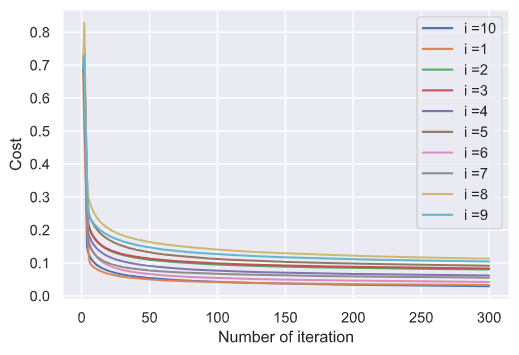
\includegraphics[scale=0.6]{gradientdescent.png}
  \caption{Cost for each iteration}
  \label{fig:gradientdescent}
\end{figure}

\subsubsection{Learning parameters using \texttt{minimize}}

This time, instead of taking gradient descent steps, you will use Scipy’s \texttt{minimize} function with CG\footnote{More details on CG method for minimize function \href{https://docs.scipy.org/doc/scipy/reference/optimize.minimize-cg.html#optimize-minimize-cg}{here}} method which is the equivalent of \texttt{fmincg} in
Octave/MATLAB.

\begin{lstlisting}
  from scipy.optimize import minimize
  lmbd = 0.1
  k = 10
  theta_optimized3 = np.zeros((k,n))
  for i in range(k):
      digitlabel = i if i else 10
      temp = minimize(fun = costFunctionReg, x0 = theta_optimized3[i],  jac = grad, args = (X, np.where(y == digitlabel,1,0).flatten(), lmbd), method='CG')
      theta_optimized3[i] = temp.x
\end{lstlisting}

\subsubsection{One-vs-all Prediction}

After training your one-vs-all classifier, you can now use it to predict the digit contained in a given image. For each input, you should compute the "probability" that it belongs to each class using the trained logistic regression classifiers. Your one-vs-all prediction function will pick the class for which the corresponding logistic regression classifier outputs the highest probability and return the class label (1, 2,..., or $K$) as the prediction for the input example.

\begin{lstlisting}[language=Python]
  def predictOneVsAll(theta, X):
    m, n = X.shape
    pred = np.dot(X, theta.T)
    return np.argmax(pred, axis=1)
\end{lstlisting}

The code in predictOneVsAll is used to use the one-vs-all classifier to make predictions. You should see that the training set accuracy is about $91.46\%$ (i.e., it classifies $91.46\%$ of the examples in the training set correctly) for the \texttt{gradientDescent} method and $96.44\%$ for the \texttt{minimize} method.

\begin{lstlisting}[language=Python]
  pred1 = predictOneVsAll(theta_optimized1, X)
  pred1 = [e if e else 10 for e in pred1]
  print(f'Training set accuracy: {np.mean(pred1 == y.flatten()) * 100:.4f}%')

  pred3 = predictOneVsAll(theta_optimized3, X)
  pred3 = [e if e else 10 for e in pred3]
  print(f'Training set accuracy: {np.mean(pred3 == y.flatten()) * 100:.4f}%')
\end{lstlisting}



\section{Neural Networks}

In the previous part of this exercise, you implemented multi-class logistic regression to recognize handwritten digits. However, logistic regression cannot form more complex hypotheses as it is only a linear classifier.\footnote{You could add more features (such as polynomial features) to logistic regression, but that can be very expensive to train.}

In this part of the exercise, you will implement a neural network to recognize handwritten digits using the same training set as before. The neural network will be able to represent complex models that form non-linear hypotheses. For this week, you will be using parameters from a neural network that we have already trained. Your goal is to implement the feedforward propagation algorithm to use our weights for prediction. In next week’s exercise, you will write the backpropagation algorithm for learning the neural network parameters.

\subsubsection{Model representation}

Our neural network is shown in Figure~\ref{fig:nn}. It has 3 layers -- an input layer, a hidden layer and an output layer. Recall that our inputs are pixel values of digit images. Since the images are of size $20 \times 20$, this gives us 400 input layer units (excluding the extra bias unit which always outputs $+1$). As before,
the training data will be loaded into the variables $X$ and $y$.

You have been provided with a set of network parameters ($\theta^{(1)}$, $\theta^{(2)}$) already trained by us. These are stored in \texttt{ex3weights.mat}. The parameters have dimensions that are sized for a neural network with 25 units in the second layer and 10 output units (corresponding to the 10 digit classes).


\begin{figure}[h!]
  \centering
  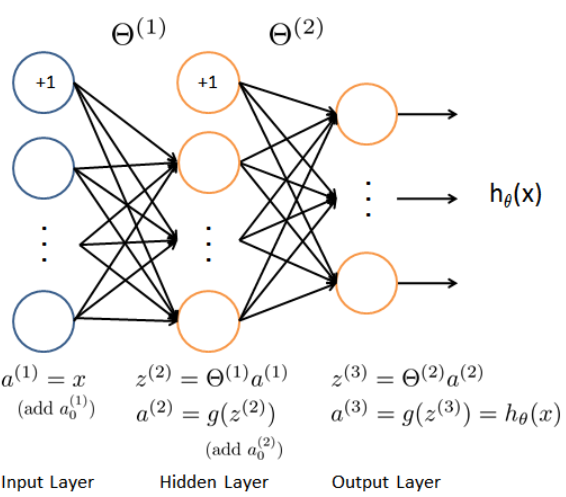
\includegraphics[scale=0.6]{nn.png}
  \caption{Neural network model}
  \label{fig:nn}
\end{figure}

\begin{lstlisting}[language=Python]
  mat2=loadmat("ex3weights.mat")
  Theta1=mat2["Theta1"]
  Theta2=mat2["Theta2"]
  print(Theta1.shape)
  print(Theta2.shape)
\end{lstlisting}

\subsubsection{Feedforward Propagation and Prediction}

Now you will implement feedforward propagation for the neural network. You should implement the feedforward computation that computes $h_\theta(x^{(i)})$ for every example $i$ and returns the associated predictions. Similar to the one-vs-all classification strategy, the prediction from the neural network will be the label that has the largest output $(h_\theta(x))_k$. You should see that the accuracy is about 97.5\%. 

\framebox[14.5cm]{\parbox{14cm}{\textbf{Implementation Note:} The matrix $X$ contains the examples in rows. When you complete the code in \texttt{predict}, you will need to add the column of 1’s to the matrix. The matrices \texttt{Theta1} and \texttt{Theta2} contain the parameters for each unit in rows. Specifically, the first row of \texttt{Theta1} corresponds to the first hidden unit in the second layer.}}


\end{document}
